\documentclass[a4paper]{article}

%====================== PACKAGES ======================

\usepackage[french]{babel}
\usepackage[utf8x]{inputenc}
%pour gérer les positionnement d'images
\usepackage{float}
\usepackage{amsmath}
\usepackage{graphicx}
\usepackage[colorinlistoftodos]{todonotes}
\usepackage{url}
%pour les informations sur un document compilé en PDF et les liens externes / internes
\usepackage{hyperref}
%pour la mise en page des tableaux
\usepackage{array}
\usepackage{tabularx}
%pour utiliser \floatbarrier
%\usepackage{placeins}
%\usepackage{floatrow}
%espacement entre les lignes
\usepackage{setspace}
%modifier la mise en page de l'abstract
\usepackage{abstract}
%police et mise en page (marges) du document
\usepackage[T1]{fontenc}
\usepackage[top=2cm, bottom=2cm, left=2cm, right=2cm]{geometry}
%Pour les galerie d'images
\usepackage{subfig}
\usepackage{svg}

%====================== INFORMATION ET REGLES ======================

%rajouter les numérotation pour les \paragraphe et \subparagraphe
\setcounter{secnumdepth}{4}
\setcounter{tocdepth}{4}

%======================== DEBUT DU DOCUMENT ========================

\begin{document}

%régler l'espacement entre les lignes
\newcommand{\HRule}{\rule{\linewidth}{0.5mm}}

%page de garde
\begin{titlepage}
\begin{center}

% Upper part of the page. The '~' is needed because only works if a paragraph has started.

\includegraphics[width=0.35\textwidth]{./logo}~\\[2cm]

\vspace{3cm}

\textsc{\LARGE INSA Lyon}\\[0.5cm]
\textsc{\Large Département Informatique}\\[0.5cm]

% Title
\HRule \\[0.4cm]

{\huge \bfseries PLD AGILE : Optimod'Lyon\\
 Rapport de fin de projet\\[0.4cm] }

\HRule \\[1.5cm]

% Author and supervisor
\begin{minipage}{0.4\textwidth}
\begin{flushleft} \large
\emph{Auteur:} H4302\\
Hazim \textsc{Asri}\\
Nihal \textsc{Boutadghart}\\
Jassir \textsc{Habba}\\
Ana \textsc{Martin}\\
Junior \textsc{Noukam}\\
Simon \textsc{Perret}\\
\end{flushleft}
\end{minipage}
\begin{minipage}{0.4\textwidth}
\begin{flushright} \large
\emph{Professeur:} \\
Mme. \textsc{Laforest}\\
\end{flushright}
\end{minipage}

\vfill

% Bottom of the page
{\large \today}

\end{center}
\end{titlepage}

~
%ne pas numéroter cette page
\thispagestyle{empty}

\tableofcontents
\thispagestyle{empty}
\setcounter{page}{0}
%ne pas numéroter le sommaire

%espacement entre les lignes d'un tableau
\renewcommand{\arraystretch}{1.5}

%====================== INCLUSION DES PARTIES ======================

~
\thispagestyle{empty}
%recommencer la numérotation des pages à "1"
\setcounter{page}{0}

\section*{Introduction} \label{ch1}
Ce document constitue le livrable de la deuxième itération de notre projet. L’objectif principal de cette phase était de faire progresser le projet en améliorant la conception initiale et en se concentrant davantage sur le développement des fonctionnalités de l’application. Lors de la première itération nous n'avons pas respecté la livraison d'une des fonctionnalités : le chargement et l'affichage de la carte. Nous avons fait le choix de déplacer la livraison de cette fonctionnalités à la deuxième itération. \\
\newline
\indent Lors de cette itération, nous avons mis à jour le diagramme de classe pour refléter les modifications apportées à l’architecture du projet et intégrer les nouvelles fonctionnalités. Nous avons également développé des modules clés, notamment le chargement des cartes et des demandes de livraison, ainsi que la gestion des livraisons dans un système complet.

\section{Mise à jour du diagramme de classe}

\begin{center}
    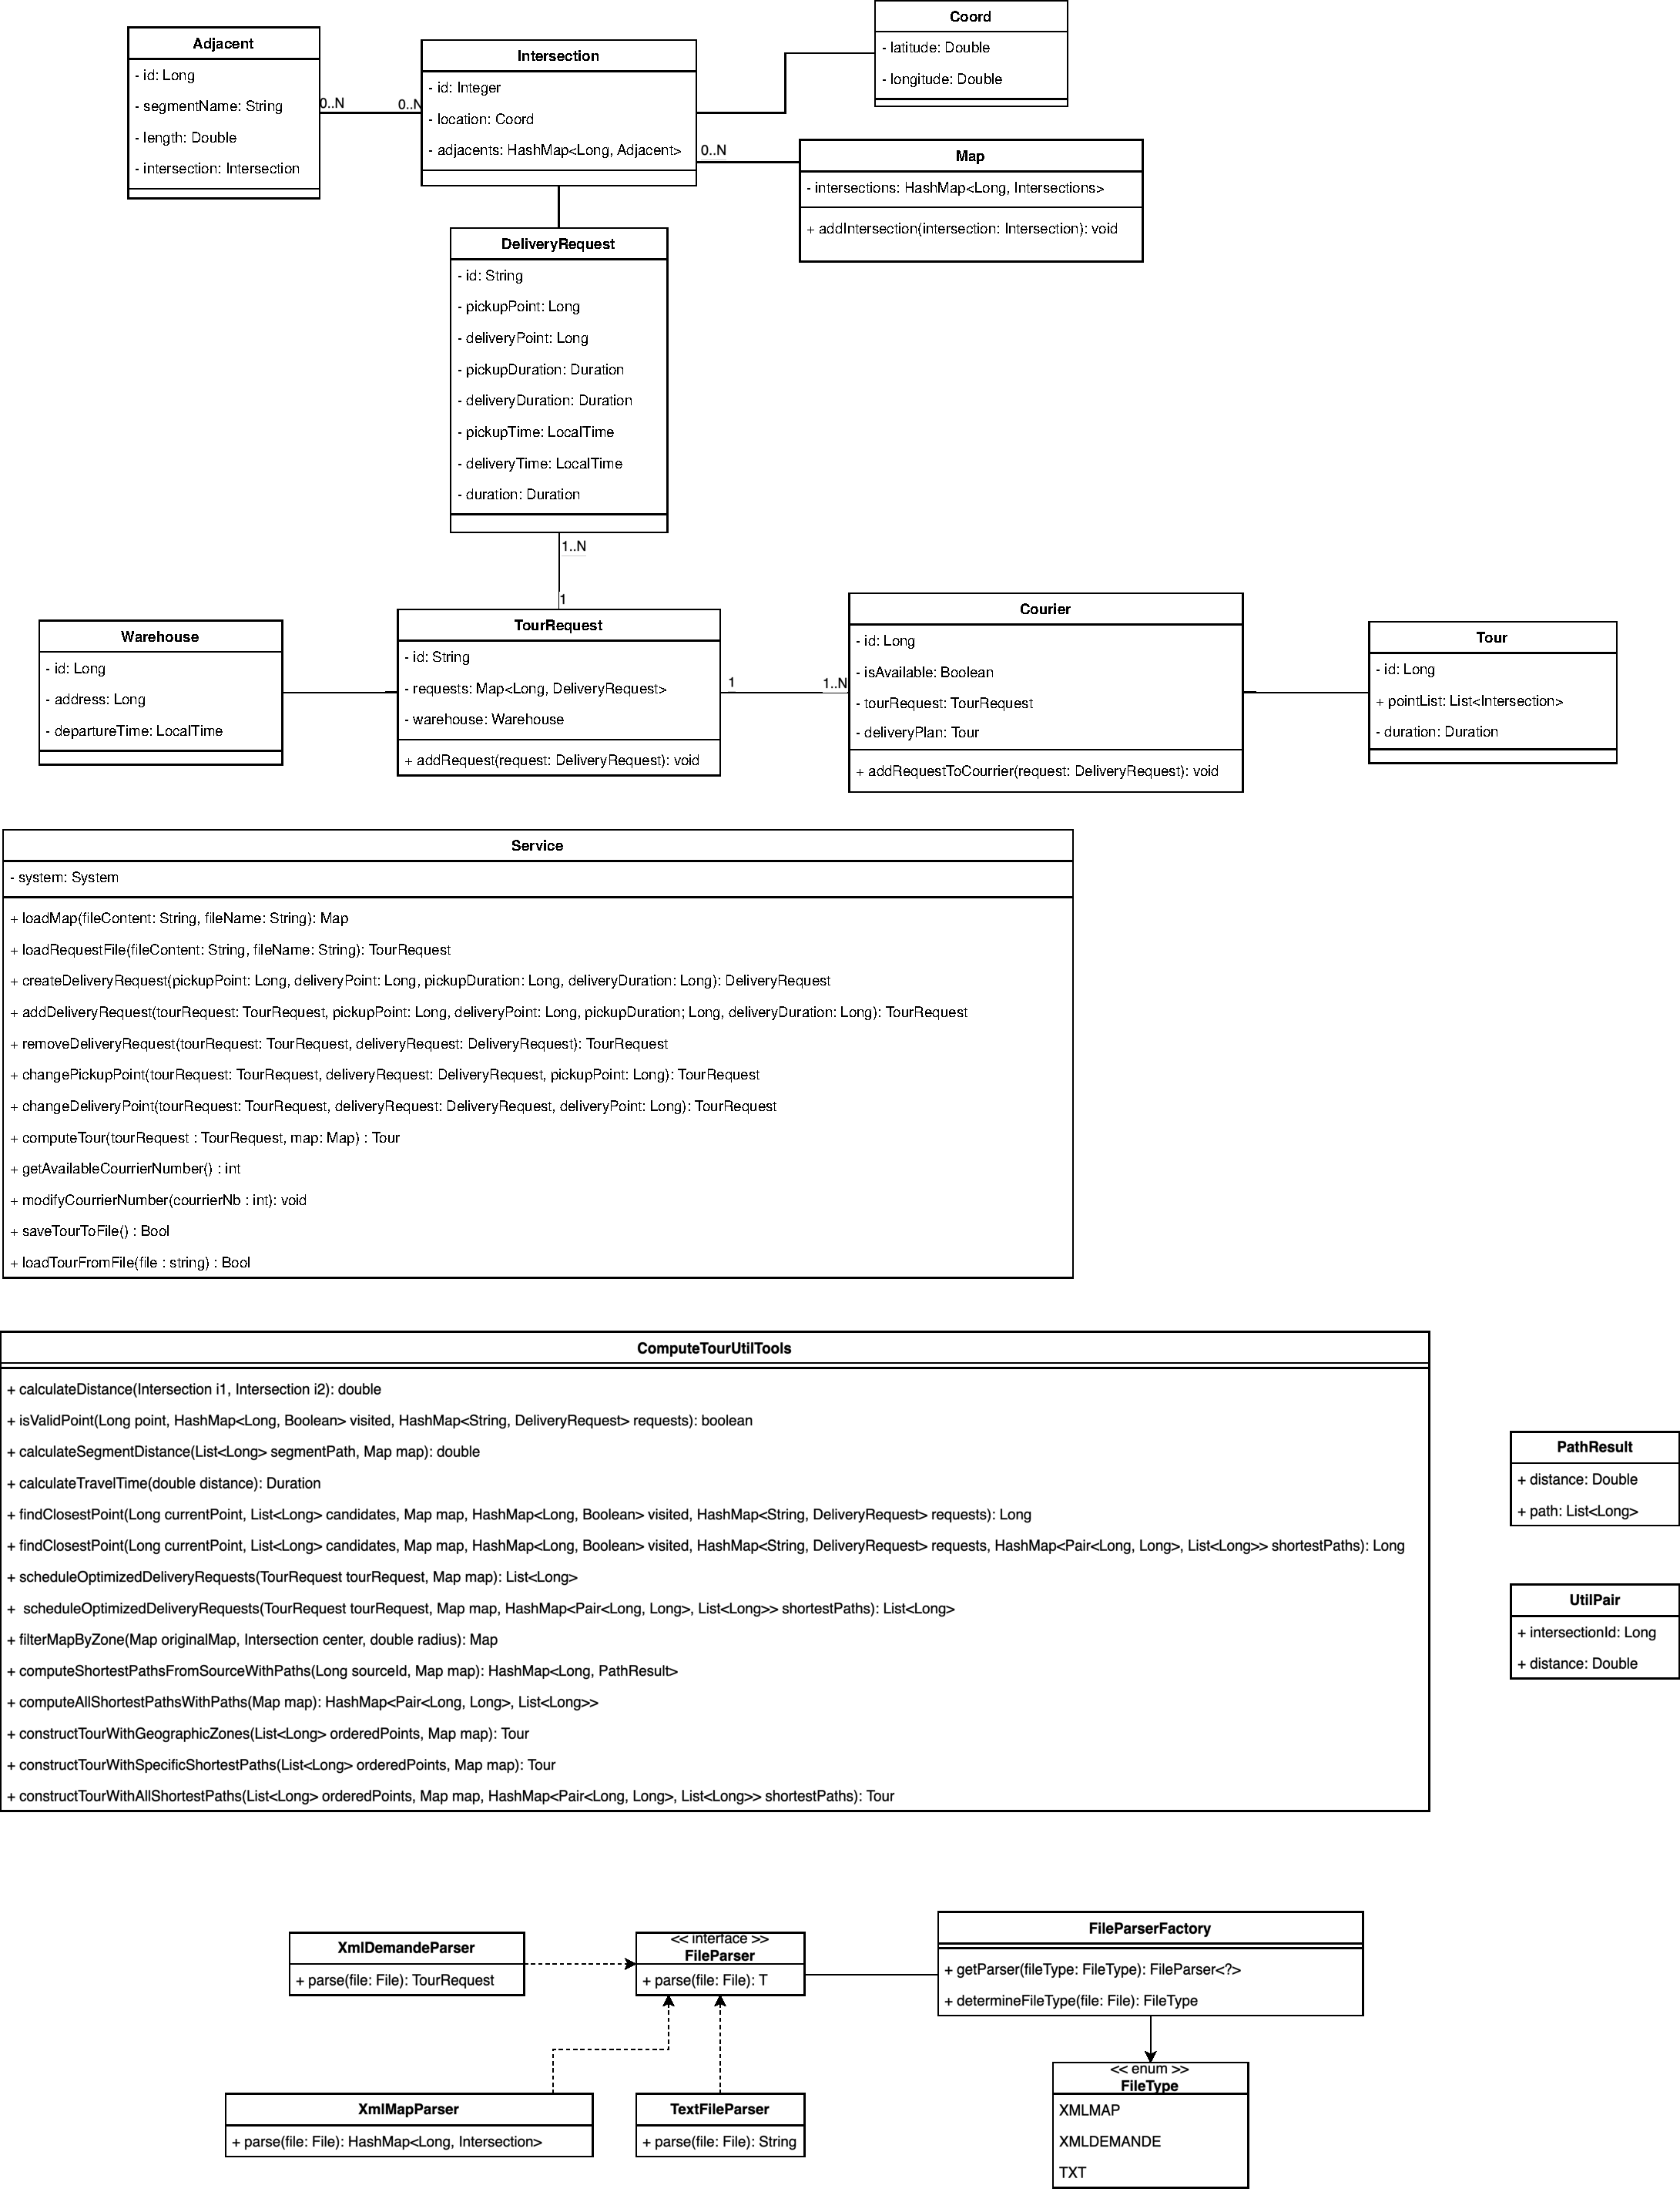
\includegraphics[width=\textwidth]{images/class.pdf}
\end{center}

Le diagramme de classe a été enrichi pour inclure de nouvelles entités et relations nécessaires au développement des fonctionnalités de l'application. Les principaux changements apportés sont les suivants :
\begin{itemize}
    \item Ajout des classes de parsage des documents xml.
    \item Ajout des classes de gestion des demandes de livraison.
    \item Ajout des classes de calcul des tournées.
\end{itemize}

\section{Développement des fonctionnalités}

Lors de cette phase, nous avons concentré nos efforts sur le développement des modules suivants :
\begin{itemize}
    \item \textbf{Chargement de la carte :} Lecture et traitement des fichiers XML pour construire le réseau modélisé par les intersections et les tronçons.
    \item \textbf{Gestion des demandes de livraison :} Création, modification, et suppression des demandes de livraison, ainsi que leur intégration dans un système de tournées.
    \item \textbf{Calcul des tournées :} Développement d’un module préliminaire permettant de calculer les itinéraires optimaux pour les livraisons.
    \item \textbf{Ajout d'une sidebar :} Barre latérale permettant d'accéder aux fonctionnalités de l'application qui seront développées lors de la dernieère itération.
    \item \textbf{API :} Ajout d'une API permettant de faire le lien entre le backend et le frontend pour charger la map.
\end{itemize}

\section{Planning des tâches}

Le tableau ci-dessous résume la répartition des tâches et la durée de leur réalisation au cours de cette itération :

\begin{table}[H]
\centering
\begin{tabularx}{\textwidth}{|X|c|c|}
\hline
\textbf{Description de la tâche} & \textbf{Durée (heure)} & \textbf{Responsable} \\ \hline
Implémenter le service de chargement de la carte            & 1                     & Junior \& Jassir                \\ \hline
Implémenter le service de calcul de tour optimal & 5                     & Junior   \\ \hline
Test unitaires pour FileManager            & 1                     & Simon \& Nihal                 \\ \hline
Implémenter service de creation de demande livraison                           & 3                    & Simon                \\ \hline
Implémenter services de modification de demande livraison                          & 1                     & Simon             \\ \hline
Implémenter d'une barre latérale                          & 8                     & Jassir             \\ \hline
Sauvegarde d'un tour dans un fichier                          & 5                     & Jassir             \\ \hline
Test unitaires pour ComputeTour                          & 1                     & Nihal             \\ \hline
Intégration CI/CD sur GitHub                         & 2                     & Ana             \\ \hline
Intégration d'une API pour le lien backend/frontend                         & 2                     & Hazim             \\ \hline
Fix bugs                         & 3                     & Hazim             \\ \hline
\end{tabularx}
\caption{Planning des tâches pour la deuxième itération}
\end{table}

\section*{Conclusion}
Cette deuxième itération a permis de poser les bases solides pour la dernière phases de développement. En mettant à jour le diagramme de classe et en concentrant nos efforts sur le développement, nous avons avancé de manière significative dans la réalisation de l’application. \\
\newline
Voici les conclusion que nous avons tiré de ce sprint :
    \begin{table}[H]
    \centering
    \begin{tabularx}{\textwidth}{|X|}
    \hline
    \textbf{Point positifs} \\ \hline
    Le repo GitHub : issues très pratiques pour connaitre les tâches de chacun \\ \hline
    Intégration très utiles du CI/CD pour éviter les erreurs au moments de merge\\ \hline
    Le backend a été lié au frontend grâce à l'API \\ \hline
    La dynamique de l'équipe permet de bien travailler en petit groupe \\ \hline
    \end{tabularx}
    \end{table}

    \begin{table}[H]
    \centering
    \begin{tabularx}{\textwidth}{|X|X|}
    \hline
    \textbf{Point négatifs} & \textbf{Axe d'amélioration} \\ \hline
    Commits pas assez régulier & Faire plusieurs commit dans une seule PR et rappeler aux autres de ne pas oublier de commit régulièrement \\ \hline
    Retard dans la livraison & Mieux plannifier le sprint et estimer les coûts \\ \hline
    Retard fréquents en début de séance & Insister pour que tout le monde soit à l'heure \\ \hline
    Sentiment de certains de ne pas s'être vu attribué de tâches utiles & Proposer plus de fonctionnalités simples à développer et communiquer avec le scrum master \\ \hline
    manque de communication au sein de l'équipe & Informer les autres quand on fait des changements important dans la structure des classes \\ \hline
    Mauvaise communication lors de la définition de la 2ème livraison & Le backend n'étant pas considéré comment livrable, ne plus l'inclure si il n'est pas lié au front \\ \hline
    Rôles de chacuns pas assez bien définis & Mieux identifier les compétences pour distribuer les tâches \\ \hline
    \end{tabularx}
    \end{table}

\end{document}